% Drawing 154/08-26 -- folder 154, batch 08, archive page 156 (PDF page 157).
% Transcription: en haut à gauche, un dessin en couleur, source de la flèche $\rho_s$ : deux configurations réunies par « ou ». Dans chacune, une droite vert clair pleine coupe deux paires de droites orange qui se croisent, avec une flèche verte vers la droite sous la droite ; à gauche la droite passe au-dessus du premier croisement (marqué d'un point, le petit triangle hachuré au crayon) et au-dessous du second, dont le triangle est marqué $T$ ; à droite elle passe au-dessous des deux croisements, le premier triangle ombré, le second marqué $T$
% Kind: two configurations joined by « ou »: a green line across two orange crossings, triangles hatched or marked T, arrow to the right (source of rho_s). Method 2 (schematic redraw from the facsimile). Status: ok.
% Notes: Top left of the page, where the curved arrow rho_s of the star diagram starts. Two configurations with « ou » between them. Left: a solid light green line, slightly arched, crosses two pairs of orange lines; it passes above the first crossing (a black dot on it; the small triangle between line and crossing hatched in pencil) and below the second, beside whose triangle T is written in pencil; a green arrow to the right under the line. Right: the same, the line passing just below both crossings; the first triangle is shaded dark, the second marked T; a short green arrow to the right. 8 orange strokes, 4 crossings, 2 green lines, 2 arrows, labels T, T, ou. Read from the 400 dpi colour scan; each pair of orange strokes fitted to the ink and drawn through its computed crossing, the triangles bounded by the computed intersections with the green line; the redraw was overlaid on the scan and agrees to within a stroke's width. The felt strokes are drawn straight (slight curvature of a few strokes not reproduced). Redrawn 2026-11-12 (issue 128): to check again.
% Coordinates: 1 unit = 1 mm = 1/100 of the crop width, same scale on both axes (bbox in page fractions: [0.328, 0.099, 0.553, 0.155]).
% Redrawn by Claude (claude-fable-5-2), issue #128, 2026-11-12; not checked by a human; not compiled (no TeX in the session).
% Rights: reproduces part of the work -- behind RENDER_TRANSCRIPTS, never published by itself.
\documentclass[tikz,border=3pt]{standalone}
\usepackage{amsmath,amssymb}
\usetikzlibrary{patterns,arrows.meta}
\tikzset{Or/.style={orange!90!black}, Lg/.style={green!60!black!70}, Br/.style={brown!80!black}, pencil/.style={black!55}, mpt/.style={circle,draw,inner sep=1.3pt}, pt/.style={circle,fill,inner sep=0.9pt}}
\colorlet{Or}{orange!90!black}\colorlet{Lg}{green!60!black!70}\colorlet{Br}{brown!80!black}
\begin{document}
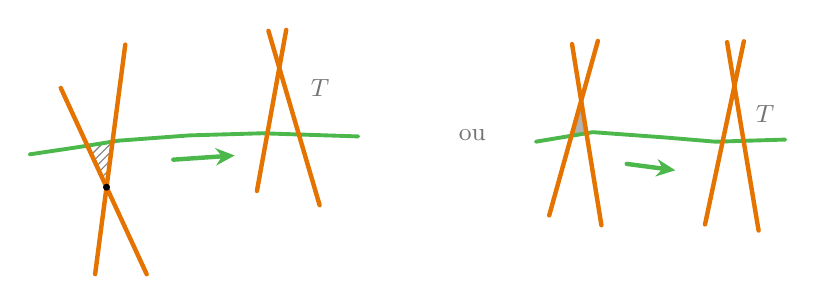
\begin{tikzpicture}[x=1mm,y=1mm,line cap=round,line join=round,font=\scriptsize]
\path[pattern=north east lines,pattern color=black!50] (11.65,-22.02) -- (12.41,-16.23) -- (9.22,-16.75) -- cycle;
\fill[black!30] (71.93,-11.04) -- (72.6,-15.17) -- (70.69,-15.49) -- cycle;
\draw[Lg,line width=1.4pt] (1.88,-17.85) -- (8.19,-16.91) -- (13.15,-16.11) -- (22.15,-15.44) -- (31.41,-15.17) -- (43.62,-15.57);
\draw[Or,line width=1.6pt] (14.03,-3.91) -- (11.65,-22.02) -- (10.2,-33.06);
\draw[Or,line width=1.6pt] (5.84,-9.42) -- (11.65,-22.02) -- (16.75,-33.07);
\node[pt] at (11.65,-22.02) {};
\draw[Lg,line width=1.6pt,-{Stealth[length=2.4mm,width=2.2mm]}] (20.13,-18.52) -- (27.92,-17.99);
\draw[Or,line width=1.6pt] (32.21,-2.16) -- (33.59,-6.86) -- (38.71,-24.3);
\draw[Or,line width=1.6pt] (34.47,-2.04) -- (33.59,-6.86) -- (30.75,-22.5);
\node[pencil,inner sep=1pt] at (38.79,-9.4) {\small $T$};
\node[pencil,inner sep=1pt] at (58.12,-15.44) {\small ou};
\draw[Lg,line width=1.4pt] (66.17,-16.24) -- (73.42,-15.03) -- (82.55,-15.7) -- (88.99,-16.24) -- (97.85,-15.97);
\draw[Or,line width=1.6pt] (70.77,-3.85) -- (71.93,-11.04) -- (74.5,-26.85);
\draw[Or,line width=1.6pt] (74.05,-3.44) -- (71.93,-11.04) -- (67.87,-25.6);
\draw[Lg,line width=1.6pt,-{Stealth[length=2.4mm,width=2.2mm]}] (77.72,-19.06) -- (83.89,-19.87);
\draw[Or,line width=1.6pt] (92.59,-3.49) -- (91.39,-9.17) -- (87.66,-26.74);
\draw[Or,line width=1.6pt] (90.46,-3.6) -- (91.39,-9.17) -- (94.46,-27.52);
\node[pencil,inner sep=1pt] at (95.3,-12.75) {\small $T$};
\end{tikzpicture}
\end{document}
